% Created 2024-08-31 Sat 10:06
% Intended LaTeX compiler: pdflatex
\documentclass[letterpaper, 12pt]{article}
\usepackage[utf8]{inputenc}
\usepackage[T1]{fontenc}
\usepackage{graphicx}
\usepackage{longtable}
\usepackage{wrapfig}
\usepackage{rotating}
\usepackage[normalem]{ulem}
\usepackage{amsmath}
\usepackage{amssymb}
\usepackage{capt-of}
\usepackage{hyperref}
\usepackage{minted}
\usepackage{xcolor}
\usepackage{hyperref}
\usepackage{tocloft}
\usepackage{minted}
\usemintedstyle{manni}
\usepackage{pdfpages}
\usepackage{fancyhdr}
\usepackage{graphicx}
\usepackage[top=1.4in, left=0.5in, right=0.5in, bottom=0.8in]{geometry}
\usepackage[T1]{fontenc}
\usepackage{helvet}
\pagestyle{fancy}
\renewcommand{\headrulewidth}{0pt}
\renewcommand{\footrulewidth}{0pt}
\setlength{\parindent}{0em}
\setlength{\parskip}{1em}
\usepackage{hyperref}
\usepackage {color}
\usepackage {tabularray}
\usepackage{xcolor}
\hypersetup{
colorlinks=true,
linkcolor=blue,
filecolor=magenta,
urlcolor=cyan,
citecolor=green,
pdfborder={0 0 0}
}
\usepackage[most]{tcolorbox}
\author{Hilduara Abreu}
\date{\today}
\title{PS192 | Cartas de Bienvenida Año Académico 2024-25\\\medskip
\large Versión en Español}
\hypersetup{
 pdfauthor={Hilduara Abreu},
 pdftitle={PS192 | Cartas de Bienvenida Año Académico 2024-25},
 pdfkeywords={},
 pdfsubject={},
 pdfcreator={Emacs 29.4 (Org mode 9.6.15)}, 
 pdflang={English}}
\begin{document}


\includepdf[pages=1,fitpaper]{/home/rob/.ps192_welcome_letters/2024/Welcome_Letters-En/pdf1.pdf}

\fancyfoot[C]{\setlength{\unitlength}{1in}\begin{picture}(5,0)\put(-1.8,-0.5){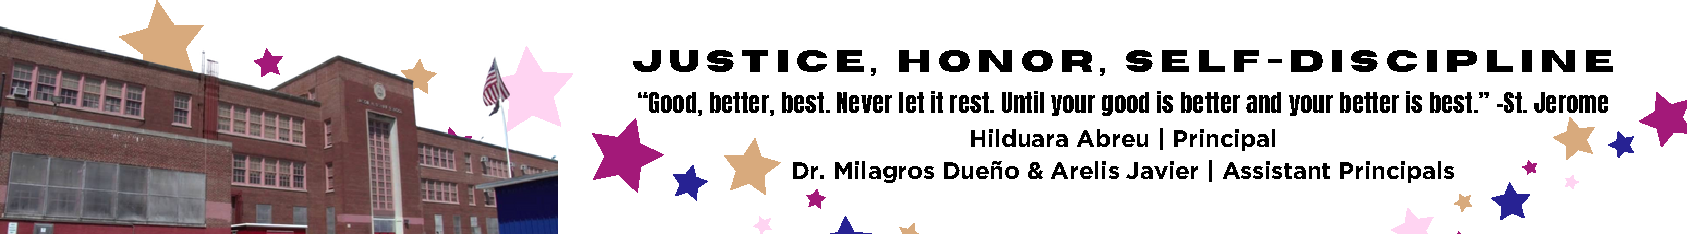
\includegraphics[width=8.8in,height=1.3in]{logo-1}}\end{picture}}
\fancyhead[C]{\setlength{\unitlength}{1in}\begin{picture}(5,0)\put(-1.9,-0.5){
\includegraphics[width=8.9in,height=1.3in]{logo-2}}\end{picture}}
\fancyhead[R]{\thepage}
\pagenumbering{gobble}

\begin{document}
\newpage
\vspace*{-0.5cm}

\section*{Tabla de Contenidos}
\label{sec:org5e5ad8e}
\begin{itemize}
\item \hyperref[sec:org4f025bc]{Introducción}
\item \hyperref[sec:orgeba5cf1]{Horario de Campana}
\item \hyperref[sec:orgefddb57]{Política de Uniformes}
\item \hyperref[sec:org2e3da0e]{Uso de Dispositivos Electrónicos}
\item \hyperref[sec:orgcc67840]{Violaciones y Acciones Disciplinarias}
\item \hyperref[sec:orgbc31239]{Carta de Bienvenida 3-K y Pre-K}
\item \hyperref[sec:orgbbbc960]{Carta de Bienvenida Grados K-5}
\item \hyperref[sec:org1f6d1e1]{Criterios de Promoción y Política de Calificación}
\item \hyperref[sec:org1ca9d51]{Directrices y Procedimientos de Seguridad y Visitantes}
\item \hyperref[sec:org71765bc]{Carta de Notificación a Padres para Escuelas Designadas para LSI}
\end{itemize}

\newpage
\vspace*{-0.5cm}

\tcbuselibrary{}
\newtcolorbox{bluebox}[1][]{
  colback=blue!5!white,
  colframe=blue!75!black,
  fonttitle=\bfseries,
  coltitle=black,
  enhanced,
  attach boxed title to top center={yshift=-2mm},
  title=#1,
  boxed title style={colback=blue!50!white}
}
\newtcolorbox{greenbox}[1][]{
  colback=green!5!white,
  colframe=green!75!black,
  fonttitle=\bfseries,
  coltitle=black,
  enhanced,
  attach boxed title to top center={yshift=-2mm},
  title=#1,
  boxed title style={colback=green!50!white}
}
\newtcolorbox{redbox}[1][]{
  colback=red!5!white,
  colframe=red!75!black,
  fonttitle=\bfseries,
  coltitle=black,
  enhanced,
  attach boxed title to top center={yshift=-2mm},
  title=#1,
  boxed title style={colback=red!50!white}
}

\section*{Introducción}
\label{sec:org4f025bc}
Estimado Padre o Tutor,

¡Bienvenido a PS 192! Estamos comprometidos a proporcionar un entorno seguro y acogedor donde cada estudiante pueda prosperar académica, social y emocionalmente. A medida que nos embarcamos en otro emocionante año escolar, es esencial que todos los miembros de nuestra comunidad escolar se mantengan informados sobre nuestras políticas, reglas, eventos y valores fundamentales. Estas pautas nos ayudan a crear un ambiente de aprendizaje positivo y productivo para nuestros estudiantes.

\begin{quote}
"La educación es el viaje donde la Justicia, el Honor y la Autodisciplina nos guían para
desbloquear nuestro máximo potencial. En PS 192, creemos en cultivar estos valores
fundamentales para inspirar grandeza en cada estudiante, padre y maestro, sentando las
bases para un futuro más brillante. Juntos, embarquémonos en este nuevo año académico
con un compromiso compartido con la excelencia y una pasión por el aprendizaje a lo largo
de la vida."  -- Hilduara Abreu
\end{quote}

En PS 192, creemos en el poder de la educación para transformar vidas. Nuestro personal dedicado trabaja incansablemente para ofrecer la educación de la más alta calidad, empoderando a nuestros estudiantes para que se conviertan en la próxima generación de pensadores y líderes que harán un impacto positivo en nuestra ciudad y más allá. Su colaboración y apoyo son cruciales en este viaje, y le agradecemos por ser una parte integral de nuestra comunidad.

Juntos, podemos asegurar que PS 192 continúe siendo un lugar donde cada niño se sienta valorado e inspirado para alcanzar su máximo potencial. Esperamos tener un año escolar exitoso y enriquecedor con su continua participación y cooperación.

Con Justicia, Honor y Autodisciplina,


\includegraphics[width=0.2\textwidth]{hil_signature}

\textbf{Hilduara Abreu, Directora}

\textbf{¡La escuela del Aprendizaje Alegre!}

\href{www.ps192.org}{www.ps192.org}
\pagebreak
\vspace*{-0.5cm}

\subsection*{Horario de Campana}
\label{sec:orgeba5cf1}
Estimado Padre o Tutor,

Un horario de campana especifica la hora de inicio y la duración de uno o más períodos de instrucción cada día de un patrón diario. Un horario diario constante y rutinas paso a paso dan a los niños un día predecible. Un horario de campana ayuda a los niños a:
\begin{itemize}
\item Sentirse en control de su entorno
\item Sentirse seguros y cómodos
\item Saber lo que está ocurriendo ahora y lo que sigue
\item Saber cómo hacer una actividad o tarea
\item Participar en el aprendizaje
\end{itemize}

Al igual que los adultos, los niños se sienten más seguros y confiados cuando sus actividades diarias son predecibles y familiares.

\begin{bluebox}[PS 192 | Horario de Campana]
\begin{table}[H]
\centering
\begin{tblr}{
  colspec={|X|X|X|X|},
  row{1}={font=\bfseries\color{MacaroniandCheese},c},
  hlines,
  vlines,
  hline{1,10} = {-}{0.08em},
}
\textbf{Período} & \textbf{Hora de Inicio} & \textbf{Hora de Fin} & \textbf{Duración} \\
1               & 08:00 AM            & 08:45 AM          & 45 minutos      \\
2               & 08:45 AM            & 09:30 AM          & 45 minutos      \\
3               & 09:30 AM            & 10:15 AM          & 45 minutos      \\
4               & 10:15 AM            & 11:05 AM          & 50 minutos      \\
5               & 11:05 AM            & 11:55 AM          & 50 minutos      \\
6               & 11:55 AM            & 12:40 PM          & 45 minutos      \\
7               & 12:40 PM            & 01:30 PM          & 50 minutos      \\
8               & 01:30 PM            & 02:15 PM          & 45 minutos
\end{tblr}
\end{table}
\end{bluebox}

\pagebreak
\vspace*{0.5cm}

Con Justicia, Honor y Autodisciplina,


\includegraphics[width=0.2\textwidth]{hil_signature}

\textbf{Hilduara Abreu, Directora}

\textbf{¡La escuela del Aprendizaje Alegre!}

\href{www.ps192.org}{www.ps192.org}

\pagebreak
\vspace*{-0.5cm}

\subsection*{Política de Uniformes}
\label{sec:orgefddb57}
\textbf{\textbf{Detalles del Uniforme}}

\begin{enumerate}
\item \textbf{Camisa Burdeos}: Todos los estudiantes deben usar una camisa de color burdeos como parte superior de su uniforme.
\item \textbf{Pantalones Azules}: Los pantalones o pantalones azul marino deben usarse como la parte inferior del uniforme.
\end{enumerate}

La política de uniformes se aplicará durante las horas escolares y en todos los eventos y actividades relacionados con la escuela, como excursiones y asambleas especiales.

\textbf{\textbf{Beneficios de la Política de Uniformes}}

Los uniformes sirven como un elemento unificador dentro de nuestra comunidad escolar y ofrecen varias ventajas significativas:

\begin{enumerate}
\item \textbf{Promover la Igualdad}: Los uniformes eliminan las disparidades socioeconómicas entre los estudiantes, asegurando que todos estén vestidos de la misma manera, independientemente de las circunstancias financieras de sus familias.
\item \textbf{Mejorar la Concentración}: El uso de uniformes reduce las distracciones relacionadas con la moda y la presión de grupo, permitiendo a los estudiantes concentrarse en sus estudios y crecimiento personal.
\item \textbf{Fomentar el Orgullo Escolar}: Un uniforme infunde un sentido de orgullo y pertenencia entre los estudiantes, ayudándolos a identificarse con y apreciar su comunidad escolar.
\item \textbf{Mejorar la Seguridad}: Los uniformes facilitan la identificación de intrusos en las instalaciones escolares, mejorando la seguridad general.
\item \textbf{Prepararse para el Éxito Futuro}: Fomentar un código de vestimenta similar a la vestimenta profesional ayuda a preparar a los estudiantes para futuras carreras donde una apariencia profesional es importante.
\end{enumerate}

\textbf{\textbf{Días de Ropa Casual}}

Entendemos que la expresión personal es importante, y por lo tanto, se programarán "Días de Ropa Casual" ocasionalmente durante el año escolar, permitiendo que los estudiantes expresen su individualidad a través de sus elecciones de vestimenta. Solicitamos amablemente su cooperación y apoyo para asegurarse de que su hijo llegue a la escuela vestido de acuerdo con nuestra política de uniformes. Creemos que esto contribuirá a un ambiente de aprendizaje más positivo y productivo para todos los estudiantes.
\pagebreak
\vspace*{-0.5cm}

\textbf{\textbf{Información de Contacto}}

Si tiene alguna pregunta o inquietud sobre la política de uniformes, no dude en comunicarse con nuestra Coordinadora de Padres, Sra. Angela Rijo, a través de los siguientes canales:
\begin{itemize}
\item Sitio web: \url{https://www.ps192.org/angela}
\item Grupo de WhatsApp
\item ClassDojo
\item Teléfono: (212) 775-9560
\item En persona durante el horario de oficina: 9:00 AM - 3:00 PM
\end{itemize}

Estamos aquí para ayudarle y apoyarle.

\textbf{\textbf{Clausura}}

Gracias por su colaboración en la creación de una comunidad de aprendizaje fuerte y vibrante en P.S. 192. Esperamos tener un año académico exitoso y enriquecedor por delante.

Con Justicia, Honor y Autodisciplina,


\includegraphics[width=0.2\textwidth]{hil_signature}

\textbf{Hilduara Abreu, Directora}

\textbf{¡La escuela del Aprendizaje Alegre!}

\href{https://www.ps192.org}{www.ps192.org}
\pagebreak
\vspace*{-0.5cm}

\subsection*{Uso de Dispositivos Electrónicos}
\label{sec:org2e3da0e}
Estimado Padre o Tutor,

\begin{redbox}[PS 192 | Política]
Dispositivos Prohibidos
Aunque no se recomienda, se permite a los estudiantes traer los siguientes artículos electrónicos a la escuela:
\begin{itemize}
\item Teléfonos celulares
\item Sistemas portátiles de música y entretenimiento (por ejemplo, iPods, reproductores de MP3)
\end{itemize}
\textit{El estudiante y/o el padre es responsable de la seguridad de estos dispositivos. La escuela no proporciona instalaciones para cargar dispositivos.}
\vspace*{3mm}

Puntos Clave Importantes:
\begin{itemize}
\item Antes de las 8:00 AM o después de las 3:35 PM en cualquier lugar dentro de la escuela donde no interrumpa las actividades educativas.
\item Estar encendidos o ser utilizados durante el tiempo de instrucción, excepto con fines educativos con la aprobación del maestro.
\item Estar encendidos o ser utilizados durante pruebas, exámenes o evaluaciones, a menos que estén explícitamente autorizados o como parte de un Programa de Educación Individualizado (IEP) o Plan de Acomodación Sección 504.
\item Estar en posesión de los estudiantes durante el horario de campana de la escuela.
\item Estar encendidos o ser utilizados durante simulacros de incendio u otros ejercicios de preparación para emergencias.
\item Ser utilizados en baños.
\item Ser utilizados durante el almuerzo en la cafetería o el patio de recreo.
\item Ser utilizados entre clases en los pasillos y escaleras.
\end{itemize}
\end{redbox}

El uso de dispositivos electrónicos debe cumplir con el Código de Disciplina del DOE, la política escolar, la Regulación A-413 del Canciller y la Política de Uso Aceptable y Seguridad en Internet del DOE (IAUSP).
\pagebreak
\vspace*{-0.2cm}

\subsection*{Violaciones y Acciones Disciplinarias}
\label{sec:orgcc67840}
Estimado Padre o Tutor,

Las violaciones de esta política pueden resultar en:
\begin{itemize}
\item Confiscación del dispositivo, con devolución solo al padre/tutor legal después de una conferencia de comportamiento.
\item Revocación del privilegio de traer artículos electrónicos a la escuela.
\item Medidas disciplinarias adicionales de acuerdo con el Código de Disciplina del DOE.
\end{itemize}

Con Justicia, Honor y Autodisciplina,


\includegraphics[width=0.2\textwidth]{hil_signature}

\textbf{Hilduara Abreu, Directora}

\textbf{¡La escuela del Aprendizaje Alegre!}

\href{www.ps192.org}{www.ps192.org}
\pagebreak
\vspace*{-1cm}

\subsection*{Carta de Bienvenida 3-K y Pre-K}
\label{sec:orgbc31239}
Estimado Padre o Tutor,

¡Estamos contando los días hasta la llegada de nuestros estudiantes el jueves 5 de septiembre de 2024! Nuestros instructores dedicados y el personal escolar están ansiosos por darle la bienvenida a lo que promete ser un año emocionante de conexiones y construcción de una comunidad sólida. Nuestros educadores atentos están emocionados de compartir sus risas, energía y pasión por el aprendizaje con sus hijos.

A medida que nos preparamos para el regreso de su hijo, queremos compartir información importante vigente en P.S. 192 para garantizar una experiencia de aprendizaje segura y agradable para todos. Por favor, tenga en cuenta las siguientes pautas:
\begin{redbox}[PS 192 | Puntos Clave para Mejorar el Aprendizaje!]
\begin{itemize}
\item Uniformes: Todos los estudiantes deben venir a la escuela diariamente vestidos con sus uniformes, que siguen siendo los mismos: una camisa burdeos y pantalones (falda, jumper) azul marino.
\item Llegada y Salida: Para garantizar un proceso de llegada y salida seguro y eficiente, por favor tome nota del siguiente horario. Habrá miembros del personal y señales que orientarán a las familias durante la primera semana de clases.
  \begin{itemize}
  \item Llegada: Patio trasero a las 8:00 AM
  \item Salida: Patio trasero a las 2:15 PM
  \end{itemize}
\item Primeros Días de Escuela: Si bien todos los estudiantes tendrán un día escolar de 8:00-2:20 PM cada día, invitamos a los padres a permanecer con sus hijos el jueves y viernes de 8:00-10:00 AM para ayudar a nuestros jóvenes estudiantes a adaptarse al ambiente escolar.
\item Útiles Escolares: P.S. 192 proporcionará todos los útiles escolares básicos, como cuadernos, carpetas y crayones. Solo pedimos que las familias de 3K y PreK proporcionen una mochila, un cambio de ropa y suministros para el tiempo de siesta diario (manta, sábana y/o un pequeño objeto de transición como una muñeca o peluche).
\end{itemize}
\end{redbox}
Nos sentimos privilegiados de ser parte de una comunidad donde padres, maestros, personal y estudiantes trabajan juntos para construir relaciones sólidas que apoyen el crecimiento académico y social. Estamos ansiosos por su participación en los diversos eventos a lo largo del año escolar y damos la bienvenida a su participación activa en el viaje educativo de su hijo.

Las actualizaciones regulares sobre eventos escolares se comunicarán a través de Nuestro Sitio Web: \href{https://www.ps192.org}{www.ps192.org}, \href{https://www.classdojo.com/}{ClassDojo}, School Messenger y nuestro grupo de WhatsApp.
\pagebreak
\vspace*{-0.1cm}

Si tiene alguna pregunta, no dude en comunicarse con nuestra Coordinadora de Padres, Angela Rijo, en
\href{mailto:arijo@schools.nyc.gov}{arijo@schools.nyc.gov}, sitio web de la escuela: \href{https://www.ps192.org/angela}{www.ps192.org/angela}, o (212) 775-9560.

Organizaremos eventos a lo largo del año y esperamos colaborar con usted tanto en persona como virtualmente. Por favor, esté atento a más información sobre todos nuestros próximos eventos:
\begin{itemize}
\item El 12 de septiembre, organizaremos Conferencias de Padres y Maestros en la noche.
\end{itemize}

Estamos emocionados de comenzar este año escolar y comprometernos con usted para asegurarnos de que su hijo disfrute de la mejor experiencia de aprendizaje posible, una en la que se sienta valorado, alentado y emocionado por aprender y sus posibilidades ilimitadas.

Me siento profundamente honrada de servir como la directora de PS 192. Gracias por su cooperación inquebrantable y dedicación a nuestros estudiantes, personal y escuela. Espero con ansias colaborar con usted en el viaje educativo de su hijo.

Con Justicia, Honor y Autodisciplina,


\includegraphics[width=0.2\textwidth]{hil_signature}

\textbf{Hilduara Abreu, Directora}

\textbf{¡La escuela del Aprendizaje Alegre!}

\href{www.ps192.org}{www.ps192.org}
\pagebreak
\vspace*{-1cm}

\subsection*{Carta de Bienvenida Grados K-5}
\label{sec:orgbbbc960}
Estimado Padre o Tutor,

A medida que nos acercamos al inicio del nuevo año escolar 2024-25, que comenzará el 5 de septiembre de 2024, extendemos una cálida bienvenida a todos nuestros estudiantes. Confiamos en que haya tenido unas vacaciones de verano agradables y saludables. Nuestro equipo dedicado y compasivo de educadores y personal escolar espera ansiosamente su regreso para lo que promete ser un año lleno de emoción, risas y aprendizaje.
\begin{greenbox}[PS 192 | Puntos Clave para Mejorar el Aprendizaje!]
\begin{itemize}
\item Uniformes: Todos los estudiantes deben venir a la escuela diariamente vestidos con sus uniformes, que siguen siendo los mismos: una camisa burdeos y pantalones (falda, jumper) azul marino.
\item Llegada y Salida: Para garantizar un proceso de llegada y salida seguro y eficiente, por favor tome nota del siguiente horario. Habrá miembros del personal y señales que orientarán a las familias durante la primera semana de clases.
\item Llegada: Nuevo este año, TODOS los estudiantes de los Grados K-5 entrarán por la Cafetería cada mañana, comenzando a las 7:40 AM para desayunar.
\item Salida: Nuevo este año, TODOS los estudiantes de los Grados K-5 serán despedidos del patio trasero a las 2:15 PM. Habrá lugares designados para cada clase por grado. Por favor, siga las señales.
\item Útiles Escolares: PS 192 proporcionará todos los útiles escolares básicos, como cuadernos, carpetas y crayones. Solo pedimos que las familias de los Grados K-5 proporcionen a los estudiantes una mochila y una caja de bolsas Ziplock de tamaño galón para que los estudiantes las usen para centros, bolsas de libros y kits de herramientas matemáticas.
\end{itemize}
\end{greenbox}
\subsubsection*{Comunidad y Eventos}
\label{sec:org6b568b7}
Nos sentimos privilegiados de ser parte de una comunidad donde padres, maestros, personal y estudiantes trabajan juntos para construir relaciones sólidas que apoyen el crecimiento académico y social. Estamos ansiosos por su participación en los diversos eventos a lo largo del año escolar y damos la bienvenida a su participación activa en el viaje educativo de su hijo. Es un honor ser parte de una comunidad donde padres, maestros, personal y estudiantes se esfuerzan colectivamente para fomentar relaciones sólidas que promuevan el crecimiento académico y social. Esperamos con ansias su participación en los eventos programados a lo largo del año escolar y
\pagebreak
\vspace*{-0.1cm}
valoramos su participación activa en la educación de su hijo.

Las actualizaciones regulares sobre los eventos escolares se comunicarán a través de Nuestro Sitio Web: \href{http://www.ps192.org}{www.ps192.org}, ClassDojo, School Messenger y nuestro grupo de WhatsApp. Si tiene alguna pregunta, no dude en comunicarse con nuestra Coordinadora de Padres, Angela Rijo, en \href{http://www.ps192.org/angela}{www.ps192.org/angela}, o (212) 775-9560.

Organizaremos eventos a lo largo del año y esperamos colaborar con usted tanto en persona como virtualmente. Por favor, esté atento a más información sobre todos nuestros próximos eventos:

\textbf{Evento Próximo}
\begin{itemize}
\item El 12 de septiembre, organizaremos nuestras Conferencias de Padres y Maestros en la noche
\end{itemize}

Estamos ansiosos por darle la bienvenida de regreso el jueves 5 de septiembre. Me siento honrada de servir como la directora de PS 192, y extiendo mi más sincero agradecimiento por su cooperación y dedicación al bienestar de nuestros hijos, personal y escuela.

Con Justicia, Honor y Autodisciplina,


\includegraphics[width=0.2\textwidth]{hil_signature}

\textbf{Hilduara Abreu, Directora}

\textbf{¡La escuela del Aprendizaje Alegre!}

\href{www.ps192.org}{www.ps192.org}
\pagebreak
\vspace*{-1cm}

\subsection*{Criterios de Promoción y Política de Calificación}
\label{sec:org1f6d1e1}
Estimado Padre o Tutor,

La Regulación A-501 del Canciller implementa una política de promoción en todo el sistema con estándares claramente definidos para la promoción en cada grado. La Política de Criterios de Promoción de P.S. 192 proporciona el proceso y los procedimientos para la implementación de esta política de promoción. Esta política es efectiva a partir del 5 de septiembre de 2024.

Esta política se promulga en el contexto de los siguientes objetivos establecidos por la Regulación A-501 del Canciller:

Todos los estudiantes de Kindergarten a 5º grado cumplirán o superarán los rigurosos estándares académicos en un plan de estudios básico basado en el desempeño. En los grados 3 a 5, todos los estudiantes cumplirán o superarán los estándares de promoción mencionados en esta regulación, y establecidos en la guía emitida por el DOE, para ser promovidos al siguiente grado y, en última instancia, estar preparados para la universidad y carreras.

\begin{itemize}
\item Toda la comunidad escolar participará continuamente en la creación y apoyo de estrategias efectivas para mejorar el rendimiento estudiantil.
\item Se utilizará un sistema integral de evaluación estudiantil, alineado con los estándares de desempeño establecidos por el Estado y la Ciudad, de manera continua para medir el progreso de los estudiantes y mejorar la instrucción en el aula.
\end{itemize}

\begin{redbox}[Sistema de Calificación de Tareas]
\begin{table}[H]
\centering
\begin{tblr}{
  colspec={|X|X|},
  row{1}={font=\bfseries\color{MacaroniandCheese},c},
  hlines,
  vlines,
  hline{1,6} = {-}{0.08em},
}
\textbf{Componente}              & \textbf{Peso} \\
Evaluaciones Internas            & 50\%            \\
Trabajo Diario en Clase           & 30\%            \\
Participación en Clase            & 10\%            \\
Proyectos                        & 5\%             \\
Tareas                        & 5\%             \\
\end{tblr}
\end{table}
\end{redbox}

\textbf{Criterios de Promoción para Grados K-2}
\begin{itemize}
\item 95 por ciento de Asistencia
\end{itemize}
\pagebreak
\vspace*{-0.1cm}
\begin{itemize}
\item Cumplir con los Estándares de Desempeño en TODAS las Materias Básicas: ELA, Matemáticas, S.S. y Ciencias. Esto significa obtener un Nivel de Desempeño 2 (una puntuación numérica de 65 por ciento) en todas las áreas de materias básicas: Lectura, Escritura, Matemáticas, Ciencias y Estudios Sociales. El promedio de los exámenes y evaluaciones de la unidad se utilizará para determinar la calificación general:
\begin{itemize}
\item Nivel 1: Un promedio agregado de 0-64 puntos
\item Nivel 2: Un promedio agregado de 65-79 puntos
\item Nivel 3: Un promedio agregado de 80-89 puntos
\item Nivel 4: Un promedio agregado de 90-100 puntos
\end{itemize}
\end{itemize}

\textbf{Lectura: Cumplir con el Benchmark de Lectura Específico del Grado DRA Mínimo}
\begin{itemize}
\item Kindergarten: Nivel de Lectura Benchmark 6 (E)
\item Primer Grado: Nivel de Lectura Benchmark 15-16 (L)
\item Segundo Grado: Nivel de Lectura Benchmark 18 (J)
\end{itemize}

\textbf{Escritura: Obtener una calificación de desempeño acumulativa de Nivel 2 en el Portafolio de Escritura}
\begin{itemize}
\item Kindergarten: 4 Piezas de Escritura (2 ficción y 2 no ficción)
\item Primer Grado: 4 Tareas de Desempeño en Escritura (2 ficción y 2 no ficción)
\item Segundo Grado: 4 Tareas de Desempeño en Escritura (2 ficción y 2 no ficción)
\end{itemize}

\textbf{Matemáticas: Obtener una calificación de desempeño acumulativa de Nivel 2. El promedio de los exámenes y evaluaciones de la unidad se utilizará para determinar la calificación general.}
\begin{itemize}
\item Nivel 1: Un promedio agregado de 0-64 puntos
\item Nivel 2: Un promedio agregado de 65-79 puntos
\item Nivel 3: Un promedio agregado de 80-89 puntos
\item Nivel 4: Un promedio agregado de 90-100 puntos
\end{itemize}
\pagebreak
\vspace*{-0.1cm}

\textbf{Tareas de Proyecto: Obtener una calificación de desempeño acumulativa de Nivel 2 en cada proyecto}
\begin{itemize}
\item Kindergarten: 3 Proyectos Individuales (Diciembre – S.S.; Febrero – Matemáticas; Abril – Ciencias)
\item Primer Grado: 3 Proyectos Individuales (Diciembre – S.S.; Febrero – Matemáticas; Abril – Ciencias)
\item Segundo Grado: 3 Proyectos Individuales (Diciembre – S.S.; Febrero – Matemáticas; Abril – Ciencias)
\end{itemize}

\textbf{Recomendación del Maestro}
\begin{itemize}
\item Análisis holístico y evidencia del trabajo en clase
\end{itemize}

\textbf{Criterios de Promoción para Grados 3-5}
\begin{itemize}
\item 95 por ciento de Asistencia
\item Cumplir con los Estándares de Desempeño en TODAS las Materias Básicas: ELA, Matemáticas, S.S. y Ciencias. Esto significa obtener un Nivel de Desempeño 2 (una puntuación numérica de 65 por ciento) en todas las áreas de materias básicas: Lectura, Escritura,
\end{itemize}

\textbf{Matemáticas, Ciencias y Estudios Sociales. El promedio de los exámenes y evaluaciones de la unidad se utilizará para determinar la calificación general:}
\begin{itemize}
\item Nivel 1: Un promedio agregado de 0-64 puntos
\item Nivel 2: Un promedio agregado de 65-79 puntos
\item Nivel 3: Un promedio agregado de 80-89 puntos
\item Nivel 4: Un promedio agregado de 90-100 puntos
\end{itemize}

\textbf{Lectura: Cumplir con el Benchmark de Lectura Específico del Grado DRA Mínimo}
\begin{itemize}
\item Tercer Grado: Nivel de Lectura Benchmark 34-38 (M-N)
\end{itemize}
\pagebreak
\vspace*{-0.1cm}

\begin{itemize}
\item Cuarto Grado: Nivel de Lectura Benchmark 38-40 (O-P)
\item Quinto Grado: Nivel de Lectura Benchmark 50 (Q-R)
\end{itemize}

\textbf{Escritura: Obtener una calificación de desempeño acumulativa de Nivel 2 en el Portafolio de Escritura}
\begin{itemize}
\item Tercer Grado: 4 Piezas de Escritura (2 ficción y 2 no ficción)
\item Cuarto Grado: 4 Tareas de Desempeño en Escritura (1 ficción y 3 no ficción)
\item Quinto Grado: 4 Tareas de Desempeño en Escritura (1 ficción y 3 no ficción)
\end{itemize}

\textbf{Matemáticas: Obtener una calificación de desempeño acumulativa de Nivel 2. El promedio de los exámenes y evaluaciones de la unidad se utilizará para determinar la calificación general.}
\begin{itemize}
\item Nivel 1: Un promedio agregado de 0-64 puntos
\item Nivel 2: Un promedio agregado de 65-79 puntos
\item Nivel 3: Un promedio agregado de 80-89 puntos
\item Nivel 4: Un promedio agregado de 90-100 puntos
\end{itemize}

\textbf{Tareas de Proyecto: Obtener una calificación de desempeño acumulativa de Nivel 2 en cada proyecto.}
\begin{itemize}
\item Tercer Grado: 3 Proyectos Individuales (Diciembre – S.S.; Febrero – Matemáticas; Abril – Ciencias)
\item Cuarto Grado: 3 Proyectos Individuales (Diciembre – S.S.; Febrero – Matemáticas; Abril – Ciencias)
\item Quinto Grado: 3 Proyectos Individuales (Diciembre – S.S.; Febrero – Matemáticas; Abril – Ciencias)
\end{itemize}

\textbf{Recomendación del Maestro}
\begin{itemize}
\item Análisis holístico y evidencia del trabajo en clase
\end{itemize}
\pagebreak
\vspace*{-0.1cm}

\textbf{Criterios de Promoción para Estudiantes del Programa de Inglés como Segundo Idioma}

Los estudiantes del Programa de Inglés como Segundo Idioma serán sujetos a los estándares de promoción basados en el número de años en las Escuelas Públicas de la Ciudad de Nueva York:
\begin{itemize}
\item Estudiantes del primer año del programa de ESL y SIFE
\begin{itemize}
\item Cumplir con los indicadores de referencia en áreas específicas como Matemáticas, S.S. y Ciencias en su idioma nativo.
\end{itemize}
\item Estudiantes del segundo y tercer año del programa de ESL
\begin{itemize}
\item Obtener un nivel 2 en la Evaluación de Matemáticas del Estado de Nueva York y realizar los avances esperados en el NYSESLAT (51 puntos dentro de un nivel de competencia)
\item Obtener al menos un puntaje de 65 por ciento (Nivel de Desempeño 2) en un mínimo de tres áreas principales.
\end{itemize}
\item Los estudiantes del cuarto año del programa de ESL serán sujetos a los mismos estándares que los estudiantes proficientes en inglés.
\end{itemize}

\textbf{Criterios de Promoción para Estudiantes de Educación Especial}
\begin{itemize}
\item Los estudiantes de Educación Especial serán sujetos a los estándares de promoción establecidos en el IEP del estudiante.
\item Un estudiante cuyo IEP no especifique criterios de promoción modificados será sujeto a los mismos criterios de promoción que los estudiantes de Educación General.
\item Los maestros utilizarán todas las evaluaciones disponibles: pruebas estandarizadas, tareas de desempeño, evaluaciones continuas del trabajo del estudiante, notas de conferencias, observaciones del maestro y juicio profesional, como un mecanismo para mejorar la instrucción en el aula y proporcionar a los padres información detallada sobre el progreso académico de su hijo.
\end{itemize}

Todos los criterios de promoción están sujetos a la aprobación final del Director. Los padres también participarán en el proceso de toma de decisiones. Los maestros mantendrán colecciones del trabajo de los estudiantes y datos formativos y sumativos que documenten el progreso de los estudiantes hacia el cumplimiento de los estándares de desempeño y los indicadores de referencia. Los maestros se reunirán con los padres regularmente para:
\pagebreak
\vspace*{-0.1cm}

\begin{itemize}
\item Nuestro personal utilizará varios métodos de comunicación para asegurarse de que los padres y tutores estén constantemente informados sobre el desarrollo social-emocional y académico de su hijo.
\begin{itemize}
\item Conferencias virtuales por Zoom o Google
\item Conversaciones telefónicas
\item Comunicación escrita, que incluye ClassDojo, correo electrónico y mensajes de texto, se utilizará para informar a los padres.
\end{itemize}
\end{itemize}

Con Justicia, Honor y Autodisciplina,


\includegraphics[width=0.2\textwidth]{hil_signature}

\textbf{Hilduara Abreu}, \textbf{Directora}

\textit{¡La Escuela del Aprendizaje Alegre!}

\href{https://www.ps192.org}{www.ps192.org}
\pagebreak
\vspace*{-1cm}

\subsection*{Directrices y Procedimientos de Seguridad y Visitantes}
\label{sec:org1ca9d51}
Estimado Padre o Tutor,

Nos complace presentar las directrices y procedimientos de nuestra estimada institución, Jacob H. Schiff/P.S. 192. Estas directrices y procedimientos han sido meticulosamente diseñados para priorizar la seguridad de todas las personas—nuestros valiosos estudiantes, dedicado personal y visitantes respetados—mientras fomentan un entorno acogedor e inclusivo. Agradecemos sinceramente su cooperación en adherirse a estos protocolos esenciales.
\begin{greenbox}[Registro de Visitantes]
\begin{itemize}
\item A su Llegada: Todos los visitantes, incluidos padres, tutores, voluntarios, contratistas e invitados estimados, deben ingresar a las instalaciones escolares por la entrada principal y proceder al escritorio del agente de seguridad para registrarse.
\item Bienvenida Cordial: Nuestro Agente de Seguridad Escolar o el personal designado dará una cálida bienvenida a todos los visitantes, preguntará sobre el propósito de su visita y solicitará una identificación con foto válida.
\item Identificación: Para garantizar la seguridad, los visitantes deben presentar una forma de identificación válida, como una licencia de conducir, identificación emitida por el gobierno, pasaporte extranjero o de EE. UU., o tarjeta de identificación consular. Posteriormente, se entregará a los visitantes una etiqueta de identificación, que deberá estar visiblemente exhibida durante toda la visita. El Agente de Seguridad Escolar ayudará a emitir la etiqueta de identificación.
\item Notificación de Asistencia: Una vez que el Agente de Seguridad Escolar o el personal designado haya completado el proceso de registro, se notificará al coordinador de padres llamando a la extensión X1190. Esto facilitará la asistencia adicional para el visitante, ya sea esperando en el vestíbulo o en el auditorio.
\item Protocolo de Salida: Se pide amablemente a los visitantes que firmen la salida con el Agente de Seguridad Escolar o el personal designado al salir del edificio. La etiqueta de identificación debe ser devuelta; la entrada principal es el punto de salida recomendado.
\end{itemize}
\end{greenbox}

\begin{itemize}
\item \textbf{Asistencia Lingüística:}
\begin{itemize}
\item Cuando un visitante no se comunique en inglés, nuestro Agente de Seguridad Escolar (SSA) o el personal escolar designado intentará identificar el idioma del visitante. Se utilizará un cartel multilingüe mostrado en el escritorio de seguridad para la identificación del idioma. Una vez que se haya determinado el idioma, el visitante será dirigido al coordinador de padres para obtener más ayuda. En casos donde no haya personal capacitado en
el idioma del visitante en el lugar,
\end{itemize}
\end{itemize}
\pagebreak
\vspace*{-0.1cm}
el coordinador de padres recurrirá a la Unidad de Interpretación Telefónica del DOE para organizar un intérprete bajo demanda.
\begin{itemize}
\item \textbf{Citas:}
\begin{itemize}
\item Política de Puertas Abiertas: Todos los martes de 2:20 a 3:00 p.m., TODOS los miembros del personal están disponibles para reunirse con los padres/tutores.
\item Visitas Programadas: Recomendamos que las visitas no urgentes se programen siempre que sea posible para asegurarnos de que los miembros del personal estén disponibles para reunirse con los visitantes y minimizar la interrupción del tiempo de instrucción. Los visitantes y el personal pueden programar citas a través de varios canales, incluidos Classdojo, correo electrónico directo del personal, nuestro sitio web escolar o contactando al coordinador de padres.
\item Llegada del Visitante: Al llegar para una cita programada, se solicita amablemente a los visitantes que sigan el mismo proceso de entrada y registro descrito anteriormente.
\end{itemize}

\item \textbf{Escolta y Supervisión:}
\begin{itemize}
\item Escolta del Visitante: Para mayor seguridad, un miembro designado del personal acompañará a los visitantes a y desde su destino previsto dentro de las instalaciones escolares, incluidas aulas, oficinas, la biblioteca, el gimnasio y otros espacios compartidos.
\item Contacto Supervisado: Los visitantes deben interactuar con los estudiantes solo si han sido autorizados expresamente por la administración escolar o como parte de un programa o evento previamente aprobado.
\end{itemize}

\item \textbf{Confidencialidad y Privacidad:}
\begin{itemize}
\item Medios y Privacidad: Para mantener la privacidad y confidencialidad de nuestros estudiantes y miembros del personal, se pide amablemente a los visitantes que no tomen fotografías ni graben videos mientras estén en las instalaciones escolares.
\item Respeto por la Privacidad: Cualquier información personal u observaciones realizadas durante la visita no deben compartirse sin el consentimiento o autorización adecuada del DOE de la Ciudad de Nueva York.
\end{itemize}

\item \textbf{Simulacros de Seguridad:}
\begin{itemize}
\item A lo largo del año académico, realizamos simulacros de seguridad para asegurarnos de que los estudiantes y el personal estén bien preparados para responder eficazmente en caso de emergencias. Estos simulacros son esenciales para la seguridad y protección de nuestra comunidad escolar e incluyen:
\pagebreak
\vspace*{-0.1cm}

\begin{itemize}
\item 12 Simulacros de Incendio: Realizados quincenalmente de septiembre a diciembre de 2024, y mensualmente después de eso.
\item 4 Simulacros de Confinamiento: Realizados cada dos meses.
\item 2 Simulacros de Emergencia en Autobús: Realizados al comienzo del año escolar y al inicio del segundo semestre (febrero de 2025).
\end{itemize}
\end{itemize}
\end{itemize}

Al seguir fielmente estas directrices y procedimientos para visitantes, todos contribuimos colectivamente a la seguridad, protección y bienestar de nuestra estimada comunidad escolar. Si tiene alguna pregunta o necesita más aclaraciones, no dude en contactarnos o ponerse en contacto con la Sra. Rijo al 646-745-0150 o 212-775-9560 X1190.

Su compromiso y apoyo inquebrantables son fundamentales para mantener un entorno de aprendizaje positivo y seguro. También está disponible asistencia adicional a través de nuestro sitio web o WhatsApp.

Una vez más, extendemos nuestro más sincero agradecimiento por su cooperación y dedicación a nuestra misión compartida.

Con Justicia, Honor y Autodisciplina,


\includegraphics[width=0.2\textwidth]{hil_signature}

\textbf{Hilduara Abreu}, \textbf{Directora}

\textit{¡La Escuela del Aprendizaje Alegre!}

\href{https://www.ps192.org}{www.ps192.org}
\newpage
\vspace*{-0.5cm}

\subsection*{Carta de Notificación a Padres para Escuelas Designadas para LSI}
\label{sec:org71765bc}
Estimado Padre o Tutor,

Esta carta es para notificarle que nuestra escuela, Jacob H. Schiff | PS 192, ha sido
designada para Apoyo y Mejora Local (LSI) por el Departamento de Educación del Estado de Nueva York (NYSED) para el año escolar 2023-24 basado en el rendimiento de nuestros estudiantes en las evaluaciones del Estado de Nueva York en el año escolar 2022-23. La
designación "Apoyo y Mejora Local (LSI)" reconoce que todas las escuelas,
incluso las de mayor rendimiento como la nuestra, están en un modo de mejora continua
y pueden beneficiarse del apoyo local de sus distritos para satisfacer las necesidades diferenciadas de los estudiantes. LSI o "Buen Estado" es el mejor estado de responsabilidad
disponible actualmente. La designación de la escuela es parte del
sistema de responsabilidad del estado de acuerdo con los requisitos federales de la Ley de Educación Primaria y Secundaria (ESEA).

Estoy segura de que los programas e intervenciones que se están implementando
en toda la ciudad y en nuestra escuela seguirán haciendo del año escolar 2023-24 una experiencia educativa de alta calidad para su hijo.

Gracias por su continua colaboración y apoyo. Todo nuestro personal escolar está
comprometido a asegurar un año exitoso para nuestros estudiantes y la comunidad escolar.
Si tiene alguna pregunta o inquietud, no dude en ponerse en contacto conmigo al 212-775-9560.

Con Justicia, Honor y Autodisciplina,


\includegraphics[width=0.2\textwidth]{hil_signature}

\textbf{Hilduara Abreu}, \textbf{Directora}

\textit{¡La Escuela del Aprendizaje Alegre!}

\href{https://www.ps192.org}{www.ps192.org}
\end{document}
